\documentclass{article}
\usepackage[top=10truemm,bottom=10truemm,left=10truemm,right=10truemm]{geometry}
\geometry{a4paper}

\usepackage{tikz}
\usetikzlibrary{shapes,arrows}
\usetikzlibrary{positioning}
\usetikzlibrary{automata, positioning}

\usepackage{newtxtext,newtxmath}

\begin{document}
\pagestyle{empty}

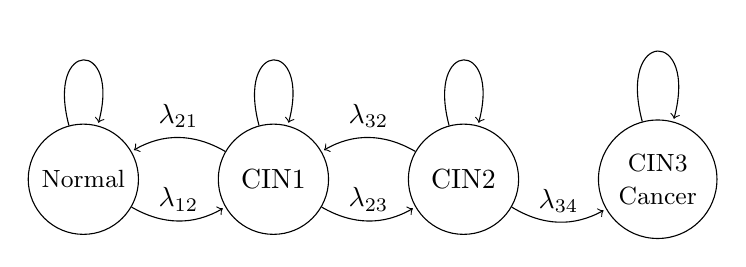
\begin{tikzpicture}
        \node[state, minimum size=1.4cm]             (1) {\small Normal};
        \node[state, minimum size=1.4cm, right=of 1] (2) {CIN1};
        \node[state, minimum size=1.4cm, right=of 2] (3) {CIN2};
        \node[state, minimum size=1.4cm, right=of 3, align=center] (4) {\small CIN3\\\small Cancer};

        \draw[every loop]
            (1) edge[bend right, auto=left]  node {$\lambda_{12}$} (2)
            (2) edge[bend right, auto=right] node {$\lambda_{21}$} (1)
            (2) edge[bend right, auto=left]  node {$\lambda_{23}$} (3)
            (3) edge[bend right, auto=right] node {$\lambda_{32}$} (2)
            (3) edge[bend right, auto=left]  node {$\lambda_{34}$} (4)
            (1) edge[loop above]             node {} (1)
            (2) edge[loop above]             node {} (2)
            (3) edge[loop above]             node {} (3)
            (4) edge[loop above]             node {} (4);
\end{tikzpicture}

\end{document}
